%%% SVN stuff
\svnidlong
{$HeadURL: https://svn.riouxsvn.com/kneadlatxinputs/ExampleArtifactFolders/7%20-%20SVD/SVD_Chapter_01.tex $}
{$LastChangedDate: 2023-12-27 21:52:08 -0500 (Wed, 27 Dec 2023) $}
{$LastChangedRevision: 44 $}
{$LastChangedBy: KneadProject $}
\svnid{$Id: SVD_Chapter_01.tex 44 2023-12-28 02:52:08Z KneadProject $}

\chapter{Scope}
\label{chap:Scope}
\DIDINFO{ALL-1.0 :: If applicable, each section has a summary of data item description (DID) information shown in this font.
These are displayed in small capital font and are not part of the formal document.
Display of these DID information notes can be turned off for formal releases, but are displayed here for reference.}



This document provides the System Version Description (\SVD) for the \ThisSystem. 
The system will be referred to as the \ThisSys.

% next line just here to add in a project specific reference
%This document is generally cited as \citeExProjSVD.
This document is generally cited as \cite{ref__KNEAD_SVD_ExProj}.

\section{Identification}
\label{sec:Identification}
\DIDINFO{ALL-1.1 :: This paragraph shall contain a full identification of the system to which this document applies, including, as applicable, identification number(s), title(s), abbreviation(s), version number(s), and release number(s).}

The \ThisSystem described in this document shall be known as \ThisSys version 1.


\section{System Overview}
\label{sec:SystemOverview}
\input{DIDINFO_Snippets/ALL/ALL_1.2_DIDINFO.tex}

The \ThisSystem system is \TBD.

Figure~\ref{fig:SystemOverview} shows the high-level architecture for the \ThisSys system. 
\begin{figure}[htbp]
	\centering
		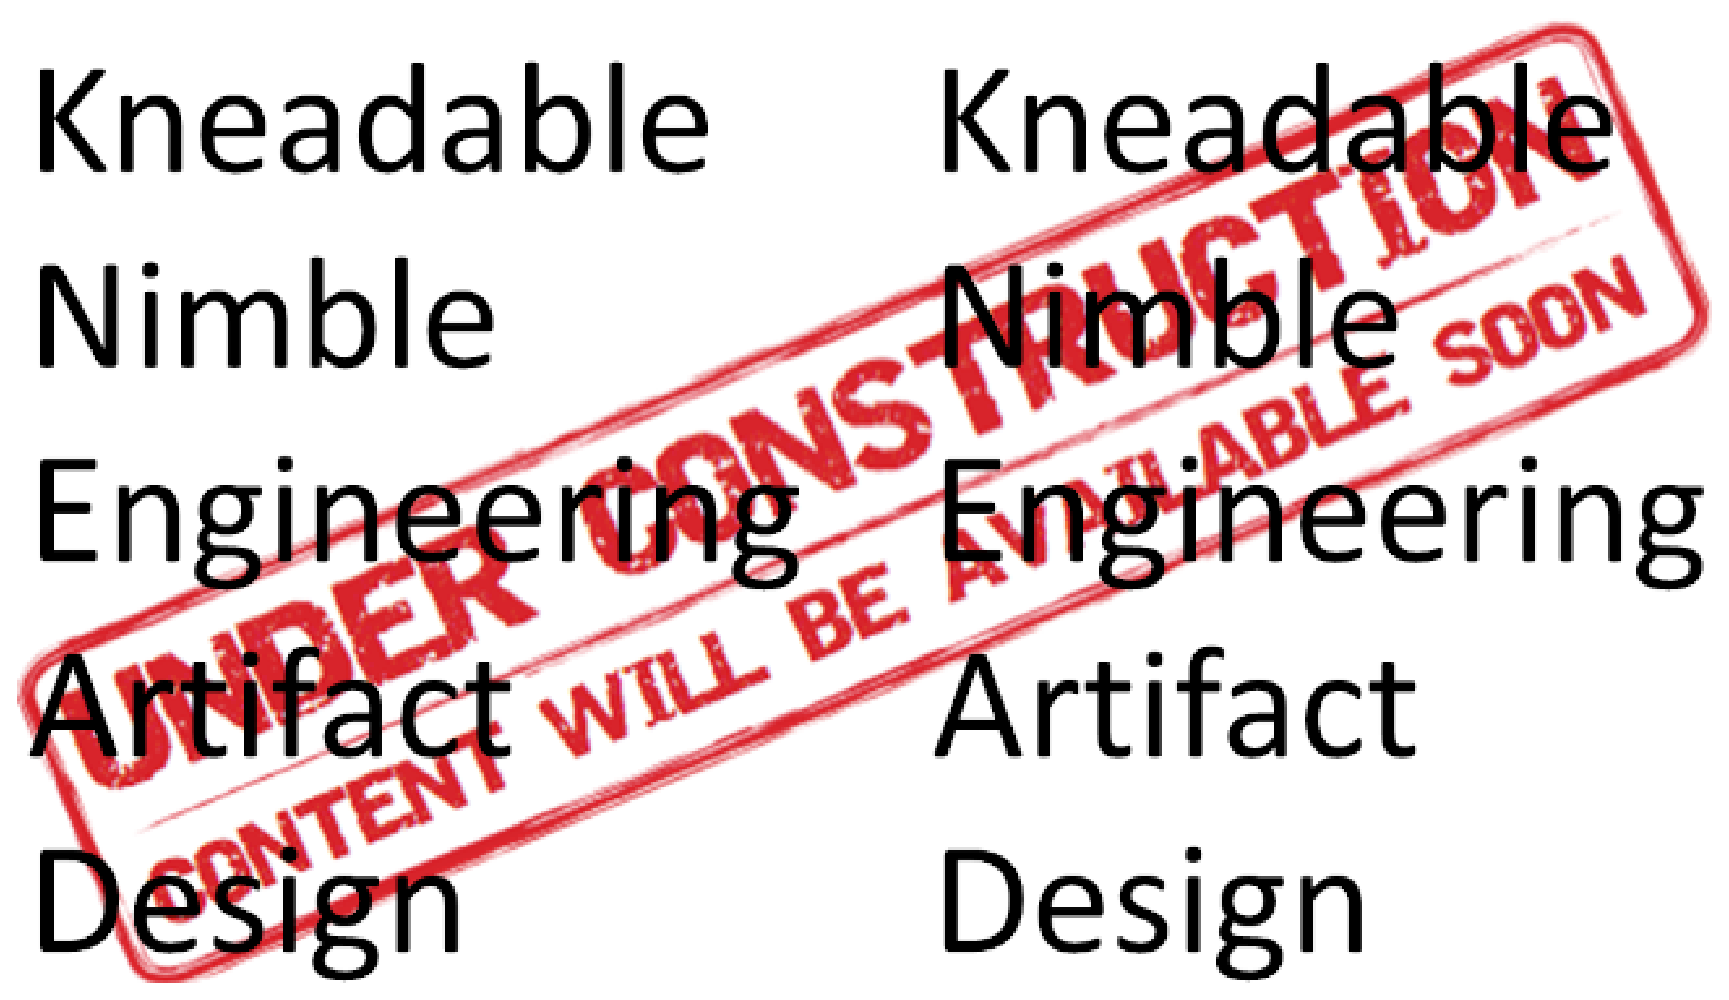
\includegraphics[width=6in]{images/KNEAD_UnderConstruction_100dpi_6.5inchesWide.eps}
		\caption{System Overview}
	\label{fig:SystemOverview}
\end{figure}
This diagram shows the major external interfaces that provide the capabilities of \ThisSys.
As are shown, the \ThisSys can provide \TBD.


The general concept of operations (\CONOP) for this system is \TBD.








\newpage
\section{Document Overview}
\label{sec:DocumentOverview}
\DIDINFO{ALL-1.3 :: This paragraph shall summarize the purpose and contents of this
document and shall describe any security or privacy considerations associated with its use.}

This section provides information about this document's security/privacy considerations, contents, structure, and version information.

%uncomment next line if the doucment is CUI
\subsection{Security and Privacy Considerations}
\label{loc:DocOverview_CUI}

%include CUI info if CUI is defined
\ifthenelse{\equal{\KNEADcuiStatus}{}}
{
	This document is not subject to \CUI restrictions.
}%endif not CUI
{% it is CUI so print CUI file info
	This document has been identified as "Controlled Unclassified Information" (\CUI).
Please follow the control block on the title page for ownership, creation, category, dissemination, and Point of Contact (\POC) information.
This information should be delineated, per \url{https://www.dodcui.mil} as:
\begin{description}[itemindent=5pt,topsep=0pt,itemsep=0pt,partopsep=0pt, parsep=0pt]
	\item[Owner] the name of the DoD Component (not required if identified in the letterhead)
	\item[Creator] identification of the office creating the document
	\item[Category] identification of the categories contained in the document
	\item[Dissemination]applicable distribution statement or limited dissemination control (LDC)
	\item[\POC]name and phone number or email of POC
\end{description}

}


\subsection{Contents and Structure}
\label{loc:DocOverview_ContentsAndStructure}

This document format is based upon the guidance in the \SDP \DID~\cite{ref__SVD_DID}, but is tailored to reflect current quality management system (\QMS) requirements for many of the items described in the \DID.
The system development plan information also follows the guidelines of ISO-12207~\cite{ref__ISO_12207} and MIL-STD-498~\cite{ref__MIL_STD_498} (from which ISO-12207 originated).
It is expected that significant coverage of the \SDP \DID items will simply be references to external \QMS or \CMMI documentation.
Thus, agencies using this artifact will formalize it to serve as a checklist for tailoring each effort per their own processes and procedures.

This tailoring also includes planning for hardware aspects as may be needed for the complete system development efforts.
The \SDP \DID mainly covered integration of software onto hardware.
This artifact includes sections that cover the development of hardware as well as development of the software.
Integration and testing are also included.
But, as noted above, all apsects of development are expected to illustrate the existing \QMS steps to be followed based on organizational processes and the project's operational needs.

This document follows a tailored \SVD sub-section order of:
\begin{description}[itemindent=5pt,topsep=0pt,itemsep=0pt,partopsep=0pt, parsep=0pt]
	\item[Section 1] provides an overview of the system and this document.
	\item[Section 2] lists general and application-specific reference documents as well as glossary terms and acronyms. 
	\item[Section 3] summarizes the required work, with references to existing \QMS processes and procedures as applicable:
	\begin{itemize}[topsep=0pt,itemsep=0pt,partopsep=0pt, parsep=0pt]
		\item program status / acquisition strategy,
		\item \SDLC Situation,
		\item plans for development of requirement artifacts,
		\item plans for overall documentation development,
		\item schedule / resource constraints, and
		\item other requirements/constraints.
	\end{itemize}
	\item[Section 4] Plans for system development
		\begin{itemize}[topsep=0pt,itemsep=0pt,partopsep=0pt, parsep=0pt]
			\item Hardware development processes and plans,
			\item Firmware development processes and plans,
			\item Software development processes and plans,
			\item Integration plans,
			\item Testing plans, and
			\item Other development activities per organizational processes.
		\end{itemize}
		\item[Section 5] Plans for system transistion
		\begin{itemize}[topsep=0pt,itemsep=0pt,partopsep=0pt, parsep=0pt]
			\item Configuration Management plans,
			\item Release plans,
			\item User Support plans, and
			\item Other system transition activities per organizational processes.
		\end{itemize}
	\item[Section 6] Management and control activities
		\begin{itemize}[topsep=0pt,itemsep=0pt,partopsep=0pt, parsep=0pt]
			\item SETR events (internal previews and with customer),
			\item Skills and resources needed,
			\item Schedule Development and Monitoring, and
			\item Other management and control activities per organizational processes.
		\end{itemize}
	\item[Section 7] if needed, lists any general notes as may be applicable.
	\item[Appendices] if needed, provide additional information as may be needed.
\end{description}

\vspace{12pt}
\DIDINFO{If this text is visible, the first instance of each section may display a summary of data item description (DID) information shown in this font.
These are displayed in small capital font and are not part of the formal document.}


%\subsection included in LaTeX_Details.tex
\subsection{Document Version Information}
\label{loc:DocOverview_LaTeXAndSvnVersionInformation}

This document was produced in \LaTeXx and \Biberx.
The editing and document preparation were performed using MiK\TeX{} version 2.9  with the build option $[$\LaTeX{}  $\Rightarrow$ PS $\Rightarrow$ PDF$]$.
The \LaTeXx {\em svn-multi} package was used to glean SVN tracking information, when files are stored in an ``SVN'' version control system.
The style {\tt \KNEADdocumentClsName}
%, which was based on the style provided in~\cite{ref__thesisguide}, 
was used to provide the \LaTeXx and \Biberx formatting details.

This revision of this document has the following properties:
\begin{table}[htbp]
	% \caption{Subversion (SVN) Data}
	% \label{tab:SVNdata}
	\centering
		\begin{tabular}{|p{1.5in}|p{4.9in}|}
		%%%%%S\multicolumn{2}{c}{\bfseries SVN Information} \\
		\hline
			{\bfseries Tracking Item}  &  {\bfseries Data} \\
		\hline		
		\hline
			Repository         & \url{\svnmainurl}  \\
		\hline
			Author         & \svnauthor  \\			
		\hline
			Revision       & \svnrev     \\	
		\hline
			Rev Date       & \svndate    \\	
		\hline	
			Print Date     & \today{} \currenttime    \\	
		\hline
			\KNEADdocumentClsName\break Version     & \KNEADdocumentClsVersion    \\	
		\hline	
			\KNEADdocumentClsName\break Date        & \KNEADdocumentClsDate   \\	
		\hline
		%%%\DocumentTexName\break Version     & \DocumentTexVersion    \\	
		%%%\hline	
		%%%\DocumentTexName\break Date        & \DocumentTexDate   \\	
		\hline						
    \end{tabular}
\end{table}
